\section{Conduction Finite Difference Solution Algorithm}\label{conduction-finite-difference-solution-algorithm}

\subsection{Basic Finite Difference Solution Approach}\label{basic-finite-difference-solution-approach}

EnergyPlus models follow fundamental heat balance principles very closely in almost all aspects of the program. However, the simulation of building surface constructions has relied on a conduction transfer function (CTF) transformation carried over from BLAST. This has all the usual restrictions of a transformation-based solution: constant properties, fixed values of some parameters, and do not produce results for the interior of the surface. As the energy analysis field moves toward simulating more advanced constructions, such as phase change materials (PCM), it becomes necessary to step back from transformations to more fundamental forms. Accordingly, a conduction finite difference (CondFD) solution algorithm has been incorporated into EnergyPlus. This does not replace the CTF solution algorithm, but complements it for cases where the user needs to simulate phase change materials or variable thermal conductivity. It is also possible to use the finite difference algorithm for zone time steps as short as one minute.

EnergyPlus includes two different options for the specific scheme or formulation used for the finite difference model.~ The first scheme is referred to as Crank-Nicholson and was the formulation used in EnergyPlus prior to version 7.~ As of version 7 a second scheme was added and is referred to as fully implicit.~ The selection between the two can be made by the user with the HeatBalanceSettings:ConductionFiniteDifference input object.~ Once selected, the same scheme is used throughout the simulation.~ Although the two different schemes differ in their fundamental heat transfer equations, they share nearly all the same supporting models for material properties, data storage, solution schemes, and spatial discretization algorithms.

The Crank-Nicholson scheme is semi-implicit and based on an Adams-Moulton solution approach. It is considered second-order in time.~ The algorithm uses an implicit finite difference scheme coupled with an enthalpy-temperature function to account for phase change energy accurately. The implicit formulation for an internal node is shown in the equation below.

\begin{equation}
C_p \rho \Delta x \frac{T_i^{j+1}-T_i^j}{\Delta t} = 
     \frac{1}{2}\left(k_W\frac{T_{i+1}^{j+1}-T_{i}^{j+1}}{\Delta x} +
                      k_E\frac{T_{i-1}^{j+1}-T_{i}^{j+1}}{\Delta x} + 
                      k_W\frac{T_{i+1}^{j}-T_{i}^{j}}{\Delta x} +
                      k_E\frac{T_{i-1}^{j}-T_{i}^{j}}{\Delta x}\right)
\end{equation}

Where:

T = node temperature

Subscripts:

i = node being modeled

i+1 = adjacent node to interior of construction

i-1 = adjacent node to exterior of construction

j+1 = new time step

j = previous time step

$\Delta$t = calculation time step

$\Delta$x = finite difference layer thickness (always less than construction layer thickness)

C\(_{p}\) = specific heat of material

k\(_{w}\) = thermal conductivity for interface between i node and i+1 node

k\(_{E}\) = thermal conductivity for interface between i node and i-1 node

$\rho$ = density of material

Then, this equation is accompanied by a second equation that relates enthalpy and temperature.

\begin{equation}
{h_i} = HTF\left( {{T_i}} \right)
\end{equation}

where HTF is an enthalpy-temperature function that uses user input data.

The fully implicit scheme is also based on an Adams-Moulton solution approach. It is considered first order in time.~ The model equation for this scheme is show in the following equation.

\begin{equation}
{C_p}\rho {\rm{\Delta x}}\frac{{T_i^{j + 1} - T_i^j}}{{{\rm{\Delta }}t}} = \left( {{k_W}\frac{{\left( {T_{i + 1}^{j + 1} - T_i^{j + 1}} \right)}}{{{\rm{\Delta x}}}} + {k_E}\frac{{\left( {T_{i - 1}^{j + 1} - T_i^{j + 1}} \right)}}{{{\rm{\Delta x}}}}} \right)
\end{equation}

For both schemes, EnergyPlus uses the following four types of nodes, as shown in the figure below (1) interior surface nodes, (2) interior nodes, (3) material interface nodes and (4) external surface nodes. The grid for each material is established by specifying a half node for each edge of a material and equal size nodes for the rest of the material. Equations such as are formed for all nodes in a construction. The formulation of all node types is basically the same.

\begin{figure}[hbtp] % fig 15
\centering
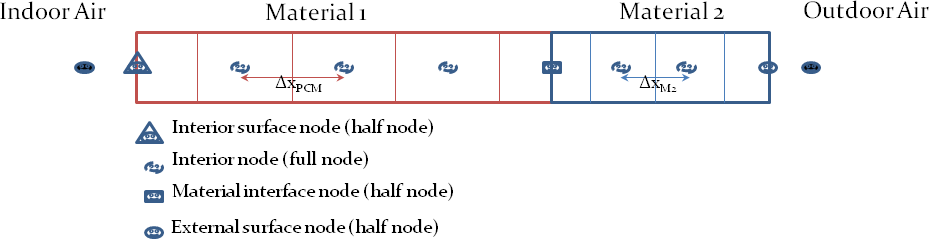
\includegraphics[width=0.9\textwidth, height=0.9\textheight, keepaspectratio=true]{media/image176.png}
\caption{Node depiction for Conduction Finite Difference Model \protect \label{fig:node-depiction-for-conduction-finite}}
\end{figure}

In the CondFD model, surface discretization depends on the thermal diffusivity of the material ($\alpha$) and time step ($\Delta$t) selected, as shown in the equation below. The default value of 3 for the space discretization constant, \emph{C}, is basically the inverse of the Fourier Number:

\begin{equation}
Fo = \frac{\alpha \Delta t}{\Delta x^2}
\end{equation}

and is based on the stability requirement for the explicit mode that requires values higher than 2, or a Fourier number lower than 0.5. However, CondFD uses implicit schemes that do not have the same stability requirements as the explicit mode. Thus, the default 3 was originally set rather arbitrary.~ As of version 7, the value of this constant can be controlled by the user with the input field called Space Discretization Constant in the HeatBalanceSettings:ConductionFiniteDifference input object.~~ The discretization method allows CondFD to assign different node spacing or grid size to different material layers in a wall or roof, as building walls and roofs typically consist of several layers of different materials having different thermal properties.

\begin{equation}
{\rm{\Delta x}} = \sqrt {{\rm{C\alpha \Delta t}}}
\end{equation}

The actual integer number of nodes for each layer is then calculated by rounding off the result from dividing the length of the material layer by the result of the equation above. After this, Δx is recalculated by dividing the length of the material by the number of nodes. A full node is equal to two half nodes. Lower values for the Space Discretization Constant yield more nodes, with higher values yield fewer nodes.

Because the solution is implicit, a Gauss-Seidell iteration scheme is used to update to the new node temperatures in the construction and under-relaxation is used for increased stability.~ The Gauss-Seidell iteration loop is the inner-most solver and is called for each surface.~ It is limited to 30 iterations but will exit early when the sum of all the node temperatures changes between the last call and the current call, normalized by the sum of the temperature values, is below ~0.000001C. This convergence criteria is typically met after 3 iterations, except when PCMs are simulated as it takes an average of 2-3 more iterations when PCM are changing phase. If the number if iterations needed to met convergence criteria start to increase, an automatic internal relaxation factor stabilities the solution and in most cases keep the number of iterations less than 10.

EnergyPlus also uses a separate, outer iteration loop across all the different inside surface heat balances so that internal long-wave radiation exchange can be properly solved.~ For CTF formulations, this iteration is controlled by a maximum allowable temperature difference of 0.002C for inside face surface temperatures from one iteration to the next (or a limit of 100 iterations). CondFD uses the same default value for allowable temperature difference as CTF. However, this parameter was found to often need to be smaller for stability and so the inside surface heat balance manager uses a separate allowable maximum temperature difference when modeling CondFD.~ The user can control the value of the relaxation factor by using the input field called~ Inside Face Surface Temperature Convergence Criteria in the HeatBalanceSettings:ConductionFiniteDifference input object. In addition, if the program detects that there is instability by watching for excessive numbers of iterations in this outer loop and may decrease the relaxation factor. Users can also output the number of iterations inside of CondFD loop for each surface and the outer internal heat balance loop for each zone with ``CondFD Inner Solver Loop Iterations'' and ``Heat Balance Inside Surfaces Calculation Iterations'' respectively.

\begin{equation}
{T_{i,new}} = {T_{i,old}} + \left( {{T_{i,new}} - {T_{i,old}}} \right)*Relax
\end{equation}

Because of the iteration scheme used for CondFD,~ the node enthalpies get updated each iteration, and then they are used to develop a variable Cp if a phase change material is being simulated. This is done by including a third equation for Cp.

\begin{equation}
Cp = \frac{{{h_{i,new}} - {h_{i,old}}}}{{{T_{i,new}} - {T_{i,old}}}}
\end{equation}

The iteration scheme assures that the correct enthalpy, and therefore the correct Cp is used in each time step, and the enthalpy of the material is accounted for accurately. Of course, if the material is regular, the user input constant Cp is used.

The algorithm also has a provision for including a temperature coefficient to modify the thermal conductivity. The thermal conductivity is obtained from:

\begin{equation}
k = {k_o} + {k_1}\left( {{T_i} - 20} \right)
\end{equation}

where:

k\(_{o}\) is the 20°C value of thermal conductivity (normal idf~ input)

k\(_{1}\) is the change in conductivity per degree temperature difference from 20°C

As of Version 7, the CondFD implementation was changed to evaluate the thermal conductivity at the interface between nodes, as shown below. In this case, EnergyPlus uses a linear interpolation between nodal points.

\begin{equation}
\medmuskip=0mu
\thinmuskip=0mu
\thickmuskip=0mu
\nulldelimiterspace=0pt
\scriptspace=0pt
{C_p}\rho {\rm{\Delta x}}\frac{{T_i^{j + 1} - T_i^j}}{{{\rm{\Delta }}t}} = \frac{1}{2}\left[ {\left( {{k_W}\frac{{\left( {T_{i + 1}^{j + 1} - T_i^{j + 1}} \right)}}{{{\rm{\Delta x}}}} + {k_E}\frac{{\left( {T_{i - 1}^{j + 1} - T_i^{j + 1}} \right)}}{{{\rm{\Delta x}}}}} \right) + \left( {{k_W}\frac{{\left( {T_{i + 1}^j - T_i^j} \right)}}{{{\rm{\Delta x}}}} + {k_E}\frac{{\left( {T_{i - 1}^j - T_i^j} \right)}}{{{\rm{\Delta x}}}}} \right)} \right]
\end{equation}

Where,

\begin{equation}
{k_W} = \frac{{\left( {k_{i + 1}^{j + 1} + k_i^{j + 1}} \right)}}{2}
\end{equation}

\begin{equation}
{{\rm{k}}_{\rm{E}}} = \frac{{\left( {{\rm{k}}_{{\rm{i}} - 1}^{{\rm{j}} + 1} + {\rm{k}}_{\rm{i}}^{{\rm{j}} + 1}} \right)}}{2}
\end{equation}

These additional property information values are put into the input file as explained in the Input/Output Reference Document, but it consists simply of a value for k1 and set of enthalpy temperature pairs that describe the enthalpy of the phase change material in straight line segments with respect to temperature.

A graph showing the effect of a large PCM on the outside surface of a zone is shown below. The phase change temperature was 30°C, and the flat temperature response during the phase change is obvious. This example was run with a zone time step of one minute to show that such small time steps can be done with the finite difference solution technique. It is more efficient to set the zone time step shorter than those used for the CTF solution algorithm. It should be set to 20 time steps per hour or greater, and can range up to 60. The finite difference algorithm actually works better with shorter zone time steps. The computation time has a minimum at a zone time step around two minutes (30 time steps/hr), and increases for shorter or longer zone time steps.

\begin{figure}[hbtp] % fig 16
\centering
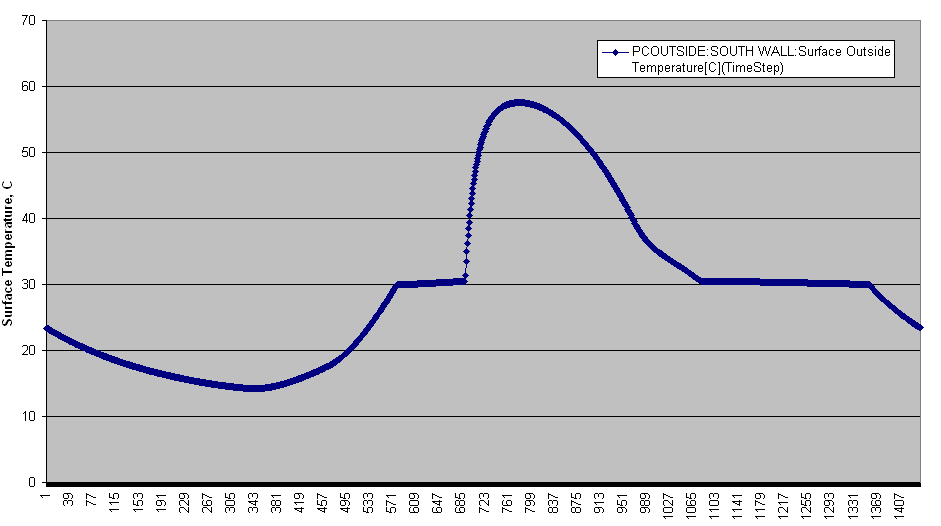
\includegraphics[width=0.9\textwidth, height=0.9\textheight, keepaspectratio=true]{media/image185.png}
\caption{Effects of Large PCM on Outside Zone Surface \protect \label{fig:effects-of-large-pcm-on-outside-zone-surface}}
\end{figure}

\subsection{Finite Difference Node Arrangement in Surfaces}\label{finite-difference-node-arrangement-in-surfaces}

The Conduction Finite Difference algorithm determines the number of nodes in each layer of the surface based on the Fourier stability criteria.~ The node thicknesses are normally selected so that the time step is near the explicit solution limit in spite of the fact that the solution is implicit. For very thin, high conductivity layers, a minimum of two nodes is used.~ This means two half thickness nodes with the node temperatures representing the inner and outer faces of the layer. All thicker layers also have two half thickness nodes at their inner and outer faces. These nodes produce layer interface temperatures.

The ConductionFiniteDifferenceSimplified capability was removed as of Version 7.2.

\subsection{Conduction Finite Difference Variable Thermal Conductivity}\label{conduction-finite-difference-variable-thermal-conductivity}

The Conduction Finite Difference algorithm has also been given the capability to use an expanded thermal conductivity function. This function, explained in the input/output document, is similar to the temperature enthalpy function. It consists of pairs of temperature and thermal conductivity values that form a linear segmented function. It is established with the MaterialProperty:VariableThermalConductivity object.

\subsection{Conduction Finite Difference Source Sink Layers}\label{conduction-finite-difference-source-sink-layers}

The Conduction Finite Difference algorithm can also invoke the source/sink layer capability by using the \textbf{Construction:InternalSource} object.

\subsection{Conduction Finite Difference Heat Flux Outputs}\label{conduction-finite-difference-heat-flux-outputs}

The Conduction Finite Difference algorithm can output the heat flux at each node and the heat capacitance of each half-node. During the CondFD solution iterations, the heat capacitance of each half node (CondFD Surface Heat Capacitance Node \textless{} n \textgreater{}) is stored:

\begin{equation}
{HeatCap_{i} = Cp_{i}*\Delta x_{i}*\rho_{i}/2}
\end{equation}

For nodes which are at the inside or outside face of the surface, there is only one half-node.

After the CondFD node temperatures have been solved for a given timestep, the heat fluxes (CondFD Surface Heat Flux Node \textless{} i \textgreater{} ) are calculated beginning with the inside face of the surface.

\begin{equation}
{QDreport_{N} = Q_{inside}}
\end{equation}

for the remaining nodes

\begin{equation}
\begin{array}{l}
QDreport_{i} = QDreport_{i+1}+HeatCap1_{i+1}* \frac{\left(T_{i+1,new}-T_{i+1,old}\right)}{\Delta t}-QSource_{i}+HeatCap2_{i} \\
\quad \quad \quad \quad * \frac{\left(T_{i,new}-T_{i,old}\right)}{\Delta t}
\end{array}
\end{equation}

Where:

HeatCap1\(_{i}\) = heat capacitance associated with a given outer half-node HeatCap2\(_{i}\) = heat capacitance associated with a given inner half-node QDreport\(_{i}\) = CondFD Surface Heat Flux Node \textless{} i \textgreater{} QSource\(_{i}\) = internal source heat flux at node i Q\(_{inside}\) = Surface Inside Face Conduction Heat Transfer Rate per Area {[}W/m\(^{2}\){]}

N = total number of nodes in a surface including the surface inside face node. Note that the variable \emph{TotNodes} used in the source code is actually N-1. The surface inside face node is referenced as \emph{TotNodes+1}.

\subsection{References}\label{references-013}

Pedersen C.O., Enthalpy Formulation of conduction heat transfer problems involving latent heat, Simulation, Vol 18, No. 2, February 1972

Versteeg, H. and Malalasekra, W. 1996. An introduction to computational fluid dynamic: the finite volume method approach. Prentice Hall.

Tabares-Velasco, P.C. and Griffith, B. 2012. Diagnostic Test Cases for Verifying Surface Heat Transfer Algorithms and Boundary Conditions in Building Energy Simulation Programs, Journal of Building Performance Simulation, doi:10.1080/19401493.2011.595501

Tabares-Velasco, P.C., Christensen, C. and Bianchi, M. 2012. Verification and Validation of EnergyPlus Phase Change Material Model for Opaque Wall Assemblies, Building and Environment 54: 186-196.
